\documentclass[11pt,a4paper]{article}
\usepackage[utf8]{inputenc}
\usepackage[english]{babel}
\usepackage[T1]{fontenc}
\usepackage{geometry}
\geometry{a4paper, margin=2.5cm}
\usepackage{parskip}
\usepackage[hyphens]{url}
\usepackage{hyperref}
\usepackage{booktabs}
\usepackage{tabularx}
\newcolumntype{L}{>{\raggedright\arraybackslash}X}
\usepackage{amsmath}
\usepackage{graphicx}
\usepackage{tikz}
\usepackage{xcolor}
\usepackage{sectsty}
\usepackage{listings}
\usetikzlibrary{shapes.geometric, arrows}

% Clean, professional monochrome colors
\definecolor{charcoal}{RGB}{44, 44, 46}       % Off-black for main body text
\definecolor{darkcharcoal}{RGB}{20, 20, 20}   % Deep black for headers
\definecolor{codebg}{RGB}{250, 250, 250}       % Very soft warm gray background for listings
\definecolor{bordergray}{RGB}{225, 225, 225}   % Soft gray for listings borders

% Apply section header coloring
\sectionfont{\color{darkcharcoal}}
\subsectionfont{\color{darkcharcoal}}
\subsubsectionfont{\color{darkcharcoal}}

% Clean, styled listings for installation commands
\lstdefinestyle{cleanstyle}{
    backgroundcolor=\color{codebg},
    frame=single,
    frameround=tttt,
    rulecolor=\color{bordergray},
    basicstyle=\ttfamily\small\color{charcoal},
    breakatwhitespace=false,         
    breaklines=true,                 
    captionpos=b,                    
    keepspaces=true,                 
    numbers=left,                    
    numberstyle=\tiny\color{gray},
    numbersep=8pt,                  
    showspaces=false,                
    showstringspaces=false,
    showtabs=false,                  
    tabsize=2
}
\lstset{style=cleanstyle}

% Monochrome hyperref settings
\hypersetup{
    hidelinks
}

\begin{document}

\color{charcoal} % Set main body text to professional charcoal color

\begin{titlepage}
    \centering
    \vspace*{1.5cm}

    % Title
    {\Huge\bfseries\color{darkcharcoal} Auditory AI \par}
    \vspace{0.6cm}
    % Subtitle
    {\Large\color{charcoal} Keyword Detection System \par}

    \vspace{2.5cm}

    % Authors
    {\large\bfseries\color{darkcharcoal} Project Team: \par}
    \vspace{0.4cm}
    {\large\color{charcoal} Mathias Kornschober (PyTorch) \par}
    {\large Dominik Praja (TensorFlow) \par}

    \vspace{1.5cm}

    % Date
    {\large\bfseries\color{darkcharcoal} Date: \par}
    \vspace{0.3cm}
    {\large\color{charcoal} June 17, 2026 \par}

    \vfill

    % School Details
    \rule{\linewidth}{0.4mm} \\[0.4cm]
    {\large\bfseries\color{darkcharcoal} Institution: \par}
    \vspace{0.3cm}
    {\large\color{charcoal} HTL Bulme \par}
    {\large Zweig Elektronik und technische Informatik \par}
    {\large Hochstamm Künstliche Intelligenz \par}
    \vspace{0.2cm}
    {\large Class: 4CHEL \par}
    {\large Supervisor: Prof. DI Schamberger Rudolf \par}
    \rule{\linewidth}{0.4mm} \\[1cm]

\end{titlepage}

\newpage
\setcounter{tocdepth}{2}
\tableofcontents

\newpage
\section{Introduction and GitHub Repository}
Voice-controlled interfaces have traditionally relied on cloud-based speech-to-text APIs, which present several challenges, including network latency, privacy concerns, and dependencies on active internet connections. The Auditory AI project was designed to address these concerns by implementing a high-performance, completely offline, on-device keyword detection system. The primary goal of the system is to capture spoken commands under a restricted vocabulary--specifically the directional and confirmation keywords \textit{yes}, \textit{no}, \textit{up}, and \textit{down}--and map them to real-time user interface actions, such as navigation or retro arcade game control (Voice Arcade).

To achieve high accessibility, the system is designed to run entirely client-side on consumer-grade hardware. Rather than relying on a heavy desktop Python environment for inference, the application utilizes WebAssembly via \texttt{onnxruntime-web} to run pre-trained convolutional neural network (CNN) graphs directly in the browser's context. Preprocessing and feature extraction--including Short-Time Fourier Transform (STFT), Mel-scale warping, and Discrete Cosine Transform (DCT-II)--are executed in a custom, pure JavaScript digital signal processing library (\texttt{dsp.js}) engineered to align exactly with standard Python audio processing packages. This architecture enables unified deployment across multiple platforms, facilitating native installations for Windows desktop, Android, and iOS using a single, decoupled HTML5/JavaScript codebase.

This document details the complete design, comparison, and implementation logs of two distinct machine learning pipelines: a PyTorch-based CNN pipeline and a TensorFlow/Keras-based CNN pipeline. Both models are optimized, exported to the open-standard ONNX format, and packaged into the frontend. Additionally, this document log details the dataset structure, model optimization benchmarks, training challenges (such as Class Imbalance and Batch Normalization instabilities), and cross-platform native compilation details.

The complete project repository containing training notebooks, model weights, native configurations, and application source code is available on GitHub at the following link:
\begin{center}
    \url{https://github.com/KOFiblto/KeywordDetection}
\end{center}

\newpage
\section{Dataset Specification and Preparation}
\subsection{Dataset Source and Licensing}
The raw audio dataset is sourced from the Kaggle mirror of the Google Speech Commands dataset (\url{https://www.kaggle.com/datasets/neehakurelli/google-speech-commands}). Although this specific mirror lists the license as unknown or unspecified on Kaggle, the original dataset was created and officially released by Pete Warden (Google Brain team) under the Creative Commons Attribution 4.0 International (CC BY 4.0) license. The CC BY 4.0 license explicitly permits redistribution, modification, and academic/commercial use under the condition that proper attribution is provided. Therefore, the dataset is safe and legally compliant for academic and educational project use.

\subsection{Restructuring and Data Pipeline}
Both PyTorch and TensorFlow pipelines train on the same shared dataset structure. An automatic download and restructuring script moves target keywords to separate directories, downsamples the negative classes, slices background noises, and creates a unified structure under a dedicated folder.

Since the raw dataset contained over 56,000 files in the \texttt{other} category (unused background noise and words), while target keywords (\textit{yes}, \textit{no}, \textit{up}, \textit{down}) only had approximately 2,000 files each, the model risked heavily over-predicting the negative class. This was resolved by downsampling the \texttt{other} category randomly to 10,000 files, splitting it in a stratified manner, and oversampling target keywords in the training split to exactly 8,000 files each using random choices with replacement. Figure~\ref{fig:dataset_distribution} shows the final sample distribution.

\begin{figure}[htbp]
    \centering
    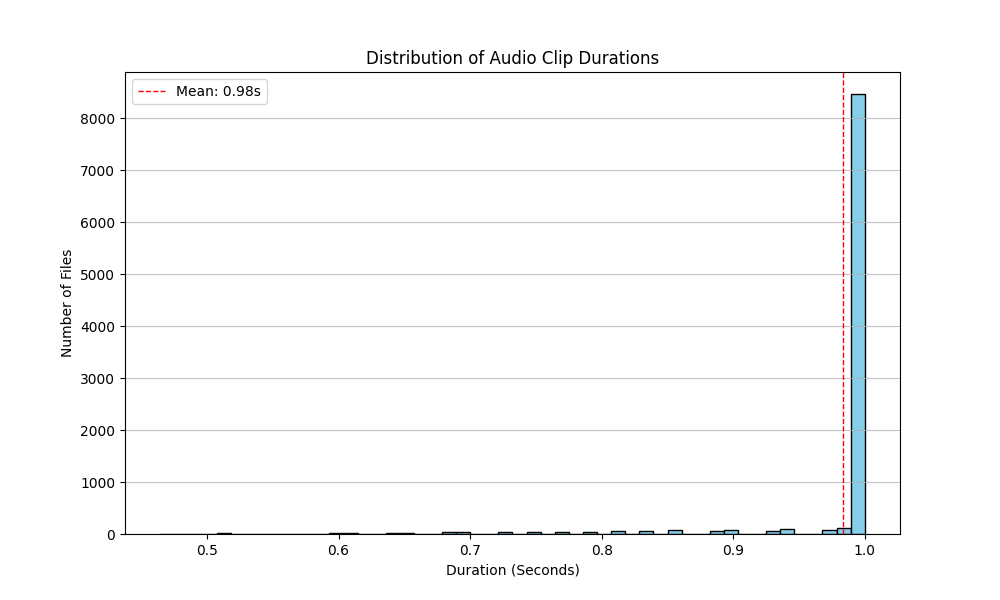
\includegraphics[width=0.75\textwidth]{../Utils/dataset_distribution.png}
    \caption{Distribution of audio samples across classes in the dataset}
    \label{fig:dataset_distribution}
\end{figure}

To filter out silent segments, ambient noise, and mislabeled utterances from the raw dataset, the project utilizes a self-written manual review application located in the \texttt{Utils/WavCleanUp} directory. This custom graphical tool provides an interface to review WAV file waveforms, calculate signal energy, and play segments, allowing developers to manually audit and prune low-quality audio files from target directories before the dataset is processed by the training pipeline.

The restructured dataset is partitioned into a stratified 3-way split consisting of 70\% training, 10\% validation, and 20\% test subsets to evaluate generalization performance.

\newpage
\section{PyTorch and TensorFlow Model Pipelines}

\subsection{Preprocessing and Feature Transformation}
Rather than feeding raw audio waveforms directly into the convolutional layers during inference, both pipelines utilize a structured feature representation. Preprocessing steps are executed in a sliding window layout:
\begin{enumerate}
    \item \textbf{Resampling}: Waveforms are resampled from the capture rate (e.g. 44.1\,kHz or 48\,kHz) to a standard 16,000\,Hz mono channel.
    \item \textbf{Short-Time Fourier Transform (STFT)}: Audio signals are divided into overlapping spectral frames.
    \item \textbf{Mel-Scale Warping}: Spectrogram frequencies are mapped onto Mel filterbanks (64 bins) to mimic human auditory perception.
    \item \textbf{Logarithmic Scaling}: Computes the logarithm of the Mel energies to align with human loudness perception.
    \item \textbf{Discrete Cosine Transform (DCT-II)}: The first 40 coefficients are extracted to obtain Mel-Frequency Cepstral Coefficients (MFCCs), decorrelating adjacent frequency bands.
\end{enumerate}

Figure~\ref{fig:spectrogram_mfcc} illustrates the visual representation of these features side-by-side.

\begin{figure}[htbp]
    \centering
    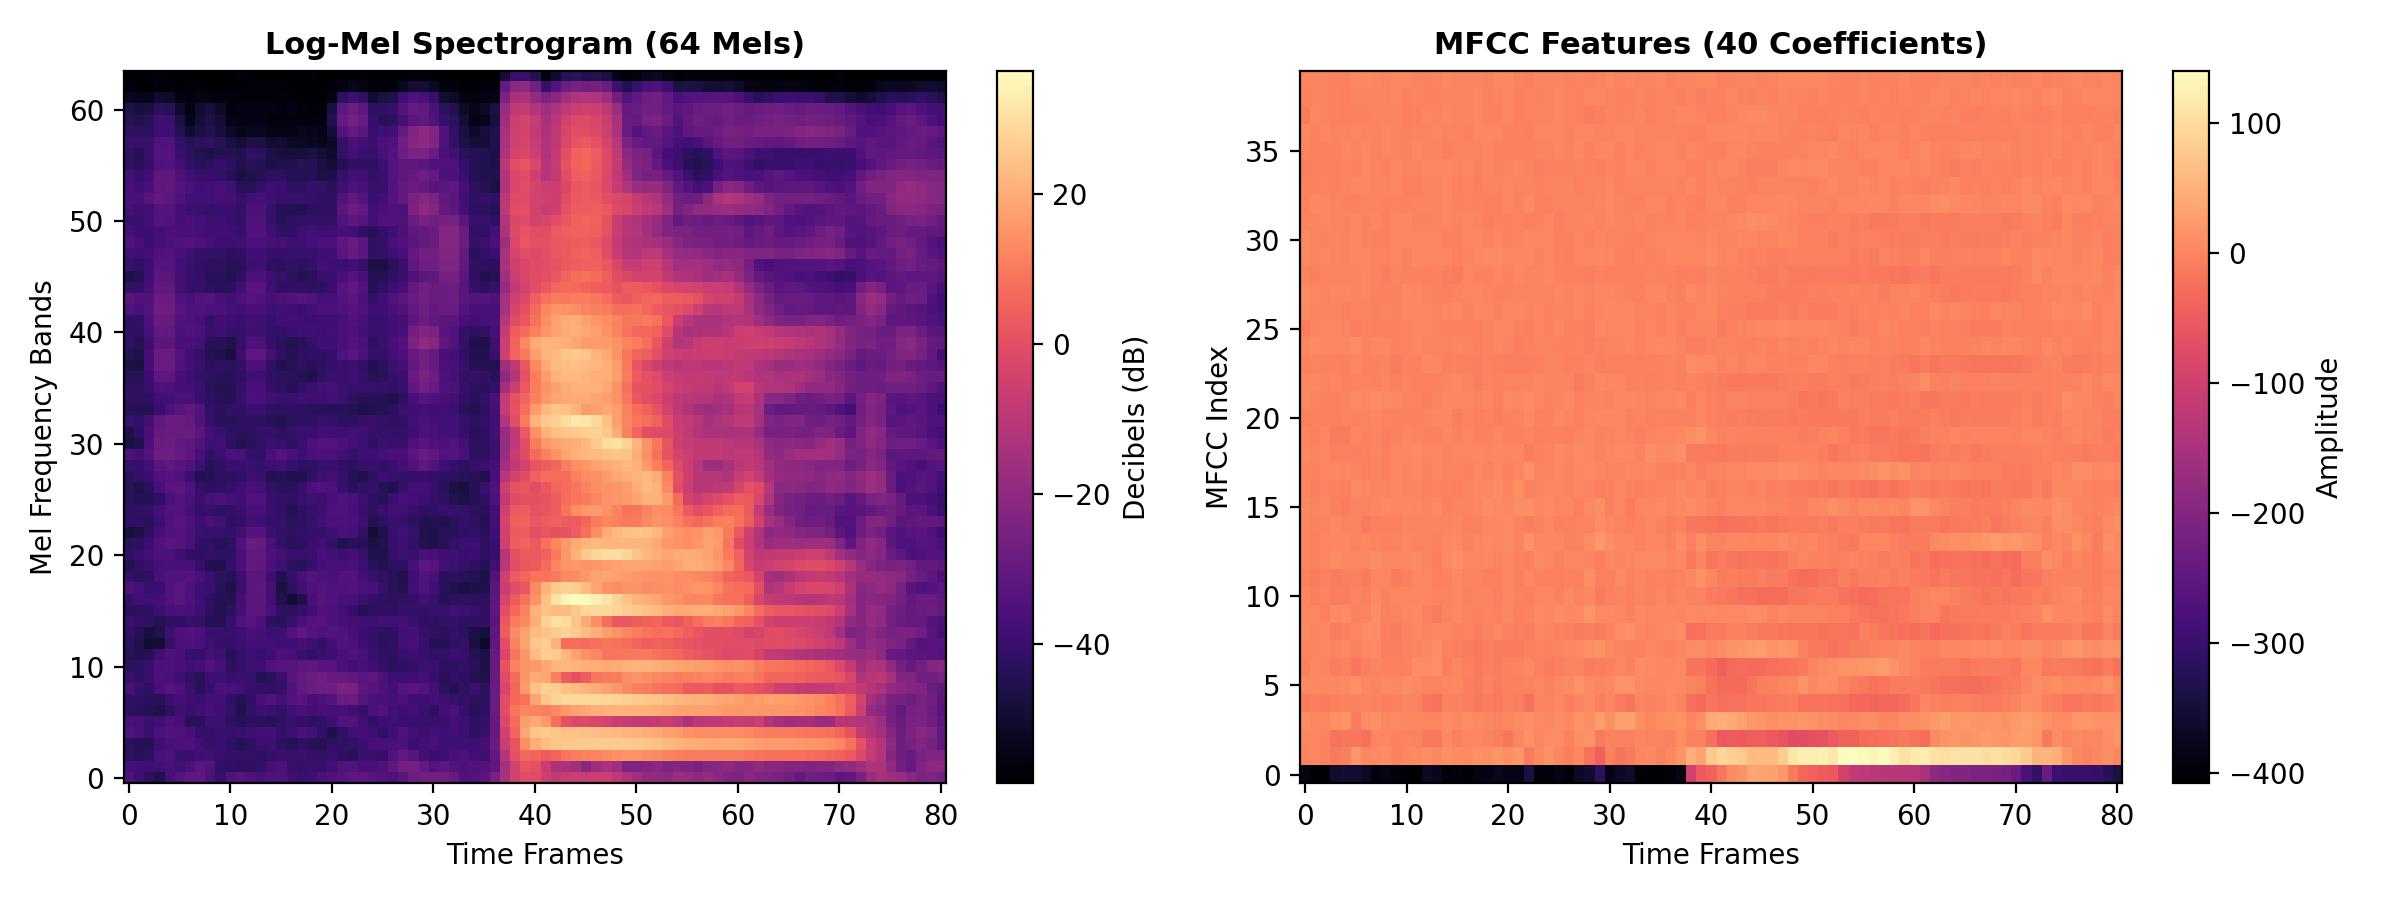
\includegraphics[width=0.95\textwidth]{spectrogram_mfcc.png}
    \caption{Log-Mel Spectrogram and MFCC features extracted from a sample audio clip}
    \label{fig:spectrogram_mfcc}
\end{figure}

\subsection{Model Architectures}
The architectures of the PyTorch and TensorFlow networks are shown in Tables~\ref{tab:pytorch_structure} and \ref{tab:tensorflow_structure}.

\begin{table}[htbp]
    \centering
    \caption{PyTorch CNN Model Structural Layout}
    \label{tab:pytorch_structure}
    \begin{tabularx}{\textwidth}{llcL}
        \toprule
        \textbf{Layer Name} & \textbf{Type}     & \textbf{Filters / Units} & \textbf{Activation / Parameters} \\
        \midrule
        Input               & -                 & -                        & Input size: $(1, 40, 81)$        \\
        Conv 1              & 2D Convolution    & 16                       & ReLU, $3 \times 3$, padding 1    \\
        Pool 1              & Max Pooling       & -                        & $2 \times 2$ pool                \\
        Conv 2              & 2D Convolution    & 32                       & ReLU, $3 \times 3$, padding 1    \\
        Pool 2              & Max Pooling       & -                        & $2 \times 2$ pool                \\
        Conv 3              & 2D Convolution    & 64                       & ReLU, $3 \times 3$, padding 1    \\
        Pool 3              & Max Pooling       & -                        & $2 \times 2$ pool                \\
        Conv 4              & 2D Convolution    & 128                      & ReLU, $3 \times 3$, padding 1    \\
        Pool 4              & Max Pooling       & -                        & $2 \times 2$ pool                \\
        Adaptive Pool       & Adaptive Avg Pool & -                        & Downscale to $4 \times 4$        \\
        Flatten             & Flatten           & -                        & Flatten to 2048                  \\
        FC 1                & Fully Connected   & 128                      & ReLU, Dropout ($p=0.3$)          \\
        FC 2 (Output)       & Fully Connected   & 5                        & Linear output                    \\
        \bottomrule
    \end{tabularx}

    \vspace{0.8cm}

    \caption{TensorFlow / Keras CNN Model Structural Layout}
    \label{tab:tensorflow_structure}
    \begin{tabularx}{\textwidth}{llcL}
        \toprule
        \textbf{Layer Name} & \textbf{Type}  & \textbf{Filters / Units} & \textbf{Activation / Parameters}     \\
        \midrule
        Input               & -              & -                        & Input size: $(40, 81, 1)$            \\
        Conv 1              & 2D Convolution & 16                       & ReLU, BN, $3 \times 3$, padding same \\
        Pool 1              & Max Pooling    & -                        & $2 \times 2$ pool                    \\
        Conv 2              & 2D Convolution & 32                       & ReLU, BN, $3 \times 3$, padding same \\
        Pool 2              & Max Pooling    & -                        & $2 \times 2$ pool                    \\
        Conv 3              & 2D Convolution & 64                       & ReLU, BN, $3 \times 3$, padding same \\
        Pool 3              & Max Pooling    & -                        & $2 \times 2$ pool                    \\
        Conv 4              & 2D Convolution & 128                      & ReLU, BN, $3 \times 3$, padding same \\
        Pool 4              & Max Pooling    & -                        & $2 \times 2$ pool                    \\
        Resizing            & Resizing       & -                        & Resize to $4 \times 4$               \\
        Flatten             & Flatten        & -                        & Flatten to 2048                      \\
        Dense 1             & Dense          & 128                      & ReLU                                 \\
        Dropout             & Dropout        & -                        & Dropout ($p=0.3$)                    \\
        Dense 2 (Output)    & Dense          & 5                        & Linear output                        \\
        \bottomrule
    \end{tabularx}
\end{table}

\subsection{ONNX Export}
Compiling and exporting both models to the ONNX format was done to enable framework-independent deployment. By packaging the weights and network graph into a standardized ONNX representation, the production frontend can execute deep learning inference directly via WebAssembly (\texttt{onnxruntime-web}). This eliminates heavy Python library dependencies (such as PyTorch or TensorFlow) in production, yielding a client-side execution latency under 5\,ms.

\subsection{Model Optimization and Milestones (PyTorch)}
The PyTorch model was optimized progressively across 11 training iterations, as documented in Table~\ref{tab:evolution}.

\begin{table}[htbp]
    \centering
    \caption{Chronological training and evaluation path}
    \label{tab:evolution}
    \begin{tabularx}{\textwidth}{llcL}
        \toprule
        \textbf{Iter.} & \textbf{Script Name}                         & \textbf{Accuracy}  & \textbf{Result and Observation}                     \\
        \midrule
        01             & \texttt{01\_specaugment.py}                  & 95.10\,\%          & Solid baseline using frequency and time masking.    \\
        02             & \texttt{02\_audio\_data\_augmentation.py}    & 95.52\,\%          & Random time-shifting improves stability.            \\
        03             & \texttt{03\_lr\_scheduler.py}                & 95.68\,\%          & ReduceLROnPlateau scheduler refines convergence.    \\
        04             & \texttt{04\_batch\_normalization.py}         & 53.95\,\%          & Severe drop (SpecAugment conflict with BatchNorm).  \\
        05             & \texttt{05\_weight\_decay.py}                & 94.89\,\%          & L2 weight decay regularizer applied.                \\
        06             & \texttt{06\_increase\_filters\_and\_mfcc.py} & 96.79\,\%          & Significant boost by switching to 40 MFCCs.         \\
        07             & \texttt{07\_increase\_mel\_bins.py}          & 89.67\,\%          & Overfitting after increasing Mel bins to 128.       \\
        08             & \texttt{08\_increase\_dropout.py}            & 95.52\,\%          & Dropout (0.3) helps regularize filters.             \\
        09             & \texttt{09\_model\_checkpointing.py}         & 95.15\,\%          & Checkpoint loading saves the best epoch parameters. \\
        10             & \texttt{10\_combined\_best.py}               & 97.95\,\%          & Combined best configurations from 1--9.             \\
        11             & \texttt{11\_combined\_stable.py}             & \textbf{98.52\,\%} & Standardized parameters for stable production.      \\
        \bottomrule
    \end{tabularx}
\end{table}

Iteration 10 (\texttt{10\_combined\_best.py}) was designed to combine the most successful configurations identified during Iterations 01 to 09. This included utilizing 40 MFCC coefficients, ReduceLROnPlateau scheduler parameters, time-shifting audio augmentations, and optimal SpecAugment boundaries. Iteration 11 (\texttt{11\_combined\_stable.py}) further standardized these features to yield the best stable accuracy for production deployment.

\subsection{Training and Evaluation Metrics}
The final training and testing metrics of the two pipelines are compared in Table~\ref{tab:metrics_comparison}.

\begin{table}[h!]
    \centering
    \caption{Comparison of training and testing metrics for PyTorch and TensorFlow}
    \label{tab:metrics_comparison}
    \begin{tabular}{lcc}
        \toprule
        \textbf{Metric}               & \textbf{PyTorch (CNN)} & \textbf{TensorFlow (Keras CNN)} \\
        \midrule
        Trained Epochs                & 40 / 40                & 100 / 100                       \\
        Final Training Loss           & 0.0858                 & 0.0515                          \\
        Final Training Accuracy       & 96.86\,\%              & 98.32\,\%                       \\
        Final Validation Accuracy     & ---                    & 97.25\,\%                       \\
        Best Test/Validation Accuracy & 98.52\,\%              & 97.46\,\%                       \\
        Final Test Accuracy           & 98.47\,\%              & 97.46\,\%                       \\
        Average Epoch Time (GPU)      & approx. 4.50\,s        & approx. 3.20\,s                 \\
        \bottomrule
    \end{tabular}
\end{table}

The training and validation accuracy progression of the PyTorch model over the training epochs is illustrated in Figure~\ref{fig:accuracy_plot}.

\begin{figure}[htbp]
    \centering
    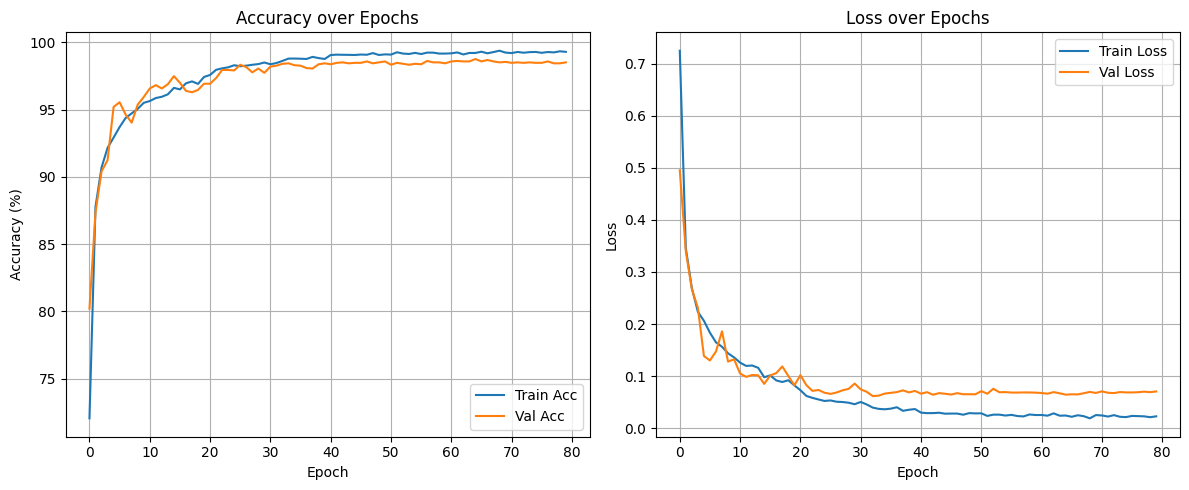
\includegraphics[width=0.75\textwidth]{AccuracyPlot.png}
    \caption{PyTorch training and validation accuracy progression over epochs}
    \label{fig:accuracy_plot}
\end{figure}

\subsection{Classification Results (Confusion Matrices)}
Figures~\ref{fig:confusion_matrix_pytorch} and \ref{fig:confusion_matrix_tensorflow} represent the confusion matrices of both pipelines evaluated against the validation test data.

\begin{figure}[htbp]
    \centering
    \begin{minipage}{0.48\textwidth}
        \centering
        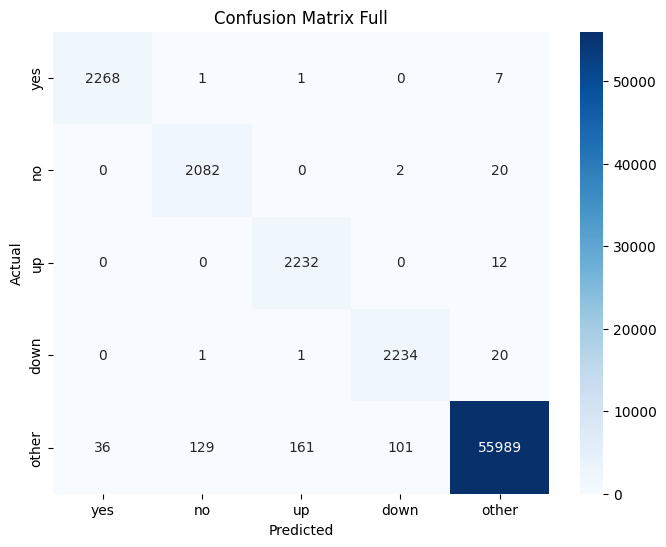
\includegraphics[width=\textwidth]{PyTorch_Confusion.png}
        \caption{PyTorch final model confusion matrix}
        \label{fig:confusion_matrix_pytorch}
    \end{minipage}
    \hfill
    \begin{minipage}{0.48\textwidth}
        \centering
        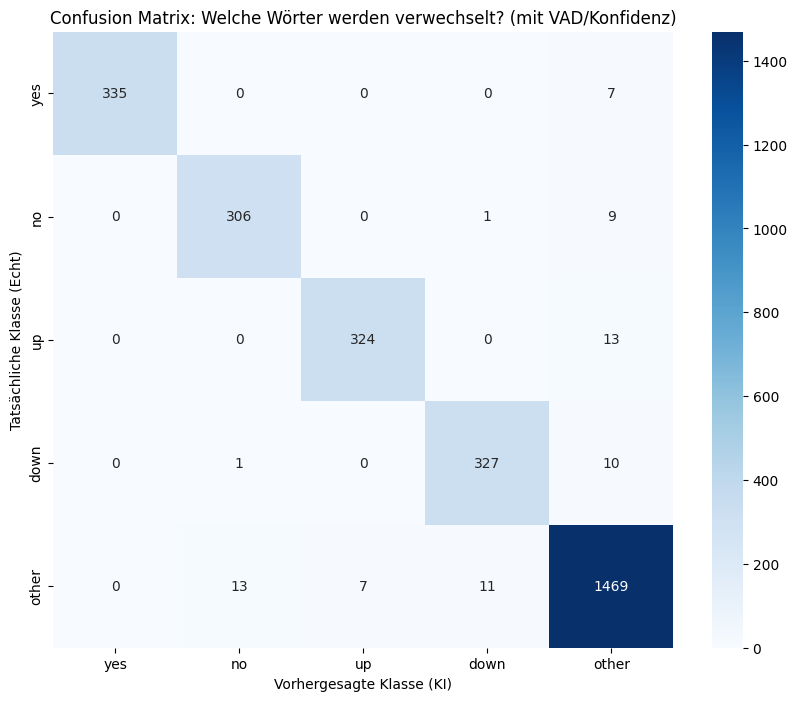
\includegraphics[width=\textwidth]{../TensorFlow/tf_confusion_matrix.png}
        \caption{TensorFlow final model confusion matrix}
        \label{fig:confusion_matrix_tensorflow}
    \end{minipage}
\end{figure}

The matrices indicate that both models display high validation separation between target command keywords, with minimal cross-classification error.

\subsection{Challenges and Resolutions}
\subsubsection{1. Batch Normalization Crash in PyTorch}
SpecAugment zero-masks entire frequency/time bands. In the PyTorch pipeline, applying Batch Normalization concurrently caused unstable running standard deviation and mean metrics, crashing validation accuracy to 53.95\%. Discarding BatchNorm for the shallow CNN solved the crash. In Keras, BatchNorm was successfully integrated because SpecAugment is only evaluated inside the training dataset pipeline and bypassed during validation model calls.

\subsubsection{2. Dynamic ONNX Shape Transposition}
PyTorch models expect a channel-first dimension layout of \texttt{[Batch,} \texttt{Channel,} \texttt{Height,} \texttt{Width]} (e.g., \texttt{[1,} \texttt{1,} \texttt{40,} \texttt{81]}), whereas TensorFlow/Keras models expect a channel-last layout of \texttt{[Batch,} \texttt{Height,} \texttt{Width,} \texttt{Channel]} (e.g., \texttt{[1,} \texttt{40,} \texttt{81,} \texttt{1]}). To maintain a unified client-side inference loop in JavaScript, the application dynamically inspects the loaded ONNX model's input signature shape. If the final dimension of the 4D shape is detected as 1, the system automatically builds a channel-last tensor layout; otherwise, it defaults to a channel-first layout. This runtime validation ensures cross-model compatibility without hardcoding model-specific inference logic.

\subsubsection{3. Poor Data Meticulosity in the Raw Dataset and Interactive Cleanup}
The Google Speech Commands raw dataset contained multiple quality defects, such as empty, silent, corrupt, or mislabeled audio files. Empty files crashed loader pipelines, while silent files caused constant false triggers in production. A custom PyQt6-based cleanup tool (\texttt{Wav\_File\_\allowbreak Cleanup.py}) was developed to calculate the RMS signal energy of all files and sort them. Quiet or corrupt files are highlighted to the developer and can be deleted or reclassified in split seconds using keyboard shortcuts.

\subsubsection{4. Extreme Class Imbalance}
Since the \texttt{other} category contained over 56,000 files (unused background noise and words), while target keywords (\textit{yes}, \textit{no}, \textit{up}, \textit{down}) only had ~2,000 files each, the model risked heavily over-predicting the negative class. This was solved by downsampling the \texttt{other} category randomly to 10,000 files, splitting it in a stratified manner (70\,\% train, 15\,\% val, 15\,\% test), and oversampling target keywords in the training split to exactly 8,000 files each using random choices with replacement.

\subsubsection{5. CPU Bottleneck during Disk I/O in Training (Resolving Memory and Disk I/O Bottlenecks)}
Initial training runs suffered from severe disk read bottlenecks: CPU usage spiked to 70--100\,\% while loading files dynamically, keeping the GPU idle and starved of data ~70\,\% of the time. This was resolved by implementing a RAM Caching strategy inside the dataset loader. All audio files are loaded once during initialization, mono-averaged, padded/cropped, and stored directly in RAM. Dynamic time-shifting is computed on-the-fly on the cached RAM tensors. Epoch training duration dropped from minutes to under 5 seconds.

\subsubsection{6. Voice Activity Detection (VAD) and Confidence Filtering}
In continuous sliding window mode (every 200\,ms), environmental typing, clicking, and breathing caused false triggers. To combat this, two filters are applied client-side:
\begin{itemize}
    \item \textbf{Voice Activity Detection (VAD)}: If the calculated root-mean-square (RMS) amplitude of the 1-second buffer falls below $0.002$, the prediction defaults to \texttt{other} without evaluating the ONNX graph.
    \item \textbf{Confidence Filtering}: If the argmax softmax probability of the model output is lower than 85\%, the detection is discarded.
\end{itemize}

\subsubsection{7. Hardware Resource Locking in the Web Browser (Audio Stream Locking)}
When hot-plugging microphones or changing input devices in the Electron GUI, the old device stream was frequently locked by the browser, causing hardware conflicts in Windows. This was resolved by iterating over all active \texttt{MediaStreamTrack} objects of the current audio stream and explicitly calling \texttt{track.stop()} to release system resources before initializing the new device stream.

\newpage
\section{Client-Side Web Application}

\subsection{Client-Side Pure JS Architecture}
To eliminate backend latency and deployment constraints, the application is fully client-side. Preprocessing and machine learning inference are performed directly inside the browser's context or web view:
\begin{itemize}
    \item \textbf{Audio Capture \& Buffer}: Captures raw audio via the browser's audio API. In Live Mode, raw samples are continuously pushed into a circular float array matching the native sample rate (e.g., 44.1\,kHz or 48\,kHz).
    \item \textbf{Resampling}: Every 200\,ms, the last 1.0 second of raw audio is read and downsampled to 16,000\,Hz using a linear interpolation helper in JavaScript.
    \item \textbf{JS Feature Extraction}: The resampled samples are transformed into MFCC (v1 models) or Log-Mel Spectrogram (v2 models) feature maps using JavaScript digital signal processing functions implemented in \texttt{dsp.js}.
    \item \textbf{WASM Inference}: The feature maps are evaluated by loading the model from the local assets folder into a web-based runtime utilizing WebAssembly.
\end{itemize}

\subsection{Interface \& Visuals}
The interface is styled using responsive CSS dark theme variables. Real-time visualizations are rendered at 60 FPS on HTML5 canvases:
\begin{enumerate}
    \item \textbf{Oscilloscope}: Renders time-domain audio amplitude.
    \item \textbf{Scrolling Spectrogram}: Renders frequency components scrolling over a 15-second history.
    \item \textbf{Timeline}: Overlays color-coded detection blocks (YES: Mint Green, NO: Soft Coral, UP: Soft Blue, DOWN: Slate Blue, OTHER: Pastel Yellow) synced with the audio.
\end{enumerate}

\subsection{Voice Arcade}
Contains five lightweight canvas games controlled by voice:
\begin{enumerate}
    \item \textbf{Flappy Bird}: Directional jumps.
    \item \textbf{Grid Runner}: Collect gems using directions.
    \item \textbf{Space Defender}: Shooter mapped to directions and shields.
    \item \textbf{Simon Memory}: Follow and repeat directional sequences.
    \item \textbf{Cyber Hi-Lo}: Card guessing game.
\end{enumerate}
Game physics are modified dynamically via a speed multiplier slider to offset vocal processing delays. The games utilize a procedural synthesizer (oscillators and gain nodes in Web Audio API) to synthesize retro sound effects locally.

\newpage
\section{Installation and Local Setup Guide}

\subsection{System Setup Requirements}
To configure and run the Auditory AI local development environment, ensure the following tools are installed on the host system:
\begin{itemize}
    \item \textbf{Node.js \& npm} (version 18 or newer)
    \item \textbf{Git}
    \item \textbf{Python} (version 3.10 to 3.12). Python 3.13 is incompatible with TensorFlow/Keras and should be avoided. A single local Python installation can support both pipelines.
\end{itemize}

First, clone the repository and change directory to the project root:
\begin{lstlisting}[language=bash]
git clone https://github.com/KOFiblto/KeywordDetection.git
cd KeywordDetection
\end{lstlisting}

\subsection{Configure PyTorch Pipeline Environment}
To run training files, audit directories, and evaluate PyTorch classifiers, establish a dedicated virtual environment and install the package requirements:
\begin{lstlisting}[language=bash]
python -m venv .venv
# Under PowerShell:
.\.venv\Scripts\Activate.ps1
# Under CMD:
.\.venv\Scripts\activate.bat

pip install -r install/pytorch/pytorch-requirements.txt
\end{lstlisting}
The dataset restructuring script can be executed next to download and prepare the Google Speech Commands files:
\begin{lstlisting}[language=bash]
python install/Download_Dataset.py
\end{lstlisting}

\subsection{Configure TensorFlow Pipeline Environment}
To compile and test Keras models, create a separate virtual environment to isolate library files, then install the TensorFlow packages and the ONNX conversion utilities:
\begin{lstlisting}[language=bash]
python -m venv .venv_tf
# Under PowerShell:
.\.venv_tf\Scripts\Activate.ps1
# Under CMD:
.\.venv_tf\Scripts\activate.bat

pip install -r install/tensorflow/tensorflow-requirements.txt
\end{lstlisting}

\subsection{Configure Frontend Node.js Dependencies}
Install the client-side packages required to launch, run, and wrap the application:
\begin{lstlisting}[language=bash]
cd frontend
npm install
cd ..
\end{lstlisting}

\subsection{Running the Application Locally}
To execute the application, run the automated startup batch file from the root folder:
\begin{lstlisting}[language=bash]
start.bat
\end{lstlisting}
This batch script calls the Node.js startup service runner (\texttt{start-services.js}), which launches the Vite server, mounts assets, and spawns the Electron app window.

If required, port conflicts and background services can be terminated by executing the cleanup batch file:
\begin{lstlisting}[language=bash]
stop.bat
\end{lstlisting}

\newpage
\section{Native Releases and Release Pipeline}
Auditory AI supports native builds and cross-platform compilation of standalone installation packages:
\begin{itemize}
    \item \textbf{Windows release package}: Executable desktop applications can be built via:
          \begin{lstlisting}[language=bash]
cd frontend
npm run dist-app
\end{lstlisting}
          This uses the \texttt{electron-builder} framework to bundle the application assets, local configurations, and ONNX models into a standalone installer (.exe) output to the \texttt{dist-app/} folder.
    \item \textbf{Mobile native projects}: Compilation is synced to native mobile directories using Capacitor.
          To sync the web assets:
          \begin{lstlisting}[language=bash]
npm run build
npx cap sync android
npx cap sync ios
\end{lstlisting}
          For Android, running \texttt{npx cap open android} opens the native package inside Android Studio. For iOS, running \texttt{npx cap open ios} opens the workspace in Xcode (macOS only).
    \item \textbf{CI/CD Release Automation}: In the production release pipeline, the Android APK compilation is executed automatically in a GitHub Actions runner using Gradle and the Android SDK command-line tools. As a result, local installations of Android Studio or Xcode are entirely optional for deployment and are only needed if developers intend to run local emulator testing.
\end{itemize}

Pre-compiled installation files, target native builds, and release assets are published and accessible on the project's GitHub Releases page:
\begin{center}
    \url{https://github.com/KOFiblto/KeywordDetection/releases}
\end{center}

\newpage
\section{Practical Insights and Lessons Learned}

\subsection{Advantage of MFCCs over Mel-Spectrograms}
Standard Mel-spectrograms retain high correlation between adjacent frequency bands. By applying the Discrete Cosine Transform (DCT) to obtain MFCCs, these bands are decorrelated. This yields a highly compact representation of speech formants, enabling the network to differentiate vocal characteristics from background noise.

\subsection{Handling Noise and SpecAugment}
Frequency masking is crucial for robust speech recognition. It forces the network to learn global word patterns even when specific bands are attenuated by cheap microphones or ambient noise. In combination with random time-shifting in the data loader, this achieves superior generalization during real-time live capture.

\subsection{Platform-Independent Inference via ONNX}
Compiling models to ONNX eliminated large deep learning library dependencies in production. Inference latency dropped to under 5\,ms per pass on a CPU, enabling highly resource-efficient deployments.

\end{document}
